\documentclass[journal,onecolumn]{IEEEtran}
\renewcommand{\baselinestretch}{1.45}

\usepackage{mathrsfs}
\usepackage{booktabs}
\usepackage{cite}
\usepackage[justification=centering]{caption} % Center the caption
\usepackage{amssymb}
\usepackage{amsmath}
\usepackage{graphics}
\usepackage{color}
\usepackage{epsfig}
\usepackage{graphicx}
\usepackage{amsthm}
\usepackage{subfigure}
\usepackage{amsmath}
\usepackage{amsfonts}
\usepackage{lettrine} % Package for dropped capital letters


\allowdisplaybreaks[4]

\title{\LARGE Data-Driven Model Free Adaptive Sliding Mode Control For Multi DC Motors Speed Regulation}

\author{Tony Blaise Bimenyimana}

\begin{document}
\maketitle

% ---------------------------------------------------------------

\begin{abstract}
    Here goes an Abstract
\end{abstract}

\section{Introduction}\label{section:1}

    \lettrine{I}n short time ago, the field of control systems experienced significant advancements, particularly in the domain of multi-agent systems. Distributed coordination of multi-agent systems has been utilized in range of practical applications, including satellite formation, autonomous, underwater vehicules,automated highway systems, and mobile robots. These applications highlight the importance and adaptability of multi-agent systems in addressing complex real world challenges.

    A critical aspect of multi-agent systems is robust speed regulation, effectively managing multi direct current (DC) motors is essential for acheiving complex machine movements. The complexity of such systems arises from the necessity to maintain synchronization and optimal performance despite parametric uncertainties and external disturbances. Conventional control methodologies, such us Proportional-Integral-Derivative (PID) control and Linear Quadratic Regulator (LQR), often fall short in these dynamic and unpredictable environments, highlighting the need for more adaptive and resilient approaches.

    Firstly, this paper aims to address these challenges by representing an innovative control strategy. Moreover, the proposed method synergizes the strengths of Model Free Adaptive Control (MFAC) and Sliding Mode Control (SMC) to achieve robust and efficient speed regulation in multi-agents systems. Secondly, By leveraging the adaptability of MFAC and the robustness of SMC, this approach seeks to enhance the performance and realibilty of multi DC motors speed regulation in the presence of uncertainties and perturbations.

    Model Free Adaptive Control (MFAC) is a technique that eschews the need for an explicit mathematical model of the system, making it highly adaptive to real time changes and disturbances. This adaptability ensures optimal control performance in varying conditions. On the other hand, Sliding Mode Control (SMC) is well known for its robustness and ability to handle Nonlinearities and uncertainties by enforcing high frequency switching control law. SMC ensures that the system states are driven to and maintained within a specified sliding surface.

    Finally, the integration of these two methodologies facilitates a control strategy that is both adaptive and resilient. MFAC continiously adjusts the control parameters based on real-time system feedback, while SMC provides a robust framework to manage system uncertainties and external disturbances. This combination is particularly well-suited for the complex dynamics and interactions inherent in multi-agent systems, offering a comprehensive solution to the challenges of robust speed control.

    The following sections will outline the remaining content of this paper:
    section 2 provides-----. Section 3 ---------------------. Section 4 presents simulation results and performance analysis , demonstrating the efficacy of the proposed method under various operating conditions.
    At the end, Section 5 concludes the paper, summarizing the key findings potential points for future research, including the extension of the proposed approach to other types of multi-agent systems and exploring further enhancements to the control algorithms.

% -----------------------------------------------------------------------------


\section{Preliminaries and problem formulation}\label{section:2}
\subsection{Preliminaries}

The set of real numbers is denoted by \(\mathbb{R}\). For a given matrix \(A \in \mathbb{R}^{n \times n}\), \(\|A\|\) represents its matrix norm. The notation \(\text{diag}(\cdot)\) refers to a diagonal matrix, and \(I\) signifies an identity matrix of appropriate dimensions. In the context of multi-agent systems, graph theory serves as a powerful tool to model interaction topologies. We will now provide a brief introduction to directed graphs within algebraic graph theory. Let \(G = (V, E, A)\) be a weighted directed graph, where \(V = \{1, 2, \ldots, N\}\) represents the set of vertices, \(E \subseteq V \times V\) denotes the set of edges, and \(A\) is the adjacency matrix. Here, \(V\) also indexes the agents. If agent \(j\) can receive a message from agent \(i\), then \((i, j) \in E\), making \(j\) the child of \(i\) and \(i\) the parent of \(j\). The neighborhood of agent \(i\) is given by \(N_i = \{j \in V \mid (j, i) \in E\}\).

The weighted adjacency matrix \(A = (a_{i,j}) \in \mathbb{R}^{N \times N}\) is defined such that \(a_{i,i} = 0\), \(a_{i,j} = 1\) if \((j, i) \in E\); otherwise, \(a_{i,j} = 0\). The Laplacian matrix of \(G\) is defined as \(L = D - A\), where \(D = \text{diag}(d_1^{\text{in}}, d_2^{\text{in}}, \ldots, d_N^{\text{in}})\) and \(d_i^{\text{in}} = \sum_{j=1}^N a_{i,j}\) is called the in-degree of vertex \(i\). A graph is said to be strongly connected if there exists a path between any pair of vertices.

\subsection{Problem Formulation}

In this research, the speed regulation problem of DC motors is frequently examined under the assumption that all motors demonstrate identical dynamic characteristics. Nevertheless, heterogeneity is still a fundamental characteristic of systems comprising multi DC motors. Even if the motors are of the same type and have similar structural features, their parameters can never be exactly the same. This inherent variability makes acheiving coordinated speed regulation across heterogeneous motors a more complex task. Let consider a multi DC motors system consisting of \(N\) motors where the interaction topology is represented by \(G\). Assume that each motor \(i\) the following nonlinear dynamics is considered:
\begin{equation}
    \label{model 1}
    y_i(k+1) = f_i(y_i(k),u_i(k)),\quad i = 1,2, \ldots, N \
\end{equation}

Where \(y_i(k) \in \mathbb{R} \) represents the output (speed of DC motor), \(u_i(k) \in \mathbb{R} \) is the control input (the voltage) and \(f_i(\cdot)\) is an unknown nonlinear function, respectively. 

We consider a scenario where multiple agents aim to track a consesus trajectory \(yd(k)\), which is exclusively accessible to a subset of agents. This trsajectory is assumed to be generated by a virtual leader designated as vertex 0. To model this interaction, we construct a direct graph \( G' = (V \cup \{0\}, E', A') \) where \( V \) denotes the set of agents, \( E' \) represents the edge set defining connections from agents to the virtual leader, and \( A' \) constitute a weighted adjacency matrix detailing these connections.

This analysis prosupposes nonlinear dynamics governing each agent's evolution. encompassing dependencies on their respective states and inputs. These nonlinear dynamics accomodate various complexities, facilitating an investigation into how agents align with the desired trajectory \(yd(k)\).

Assumption 1: The partial derivative of the nonlinear function \( f_i(\cdot) \) with respect to \( u_i(k) \) is continuous.

Assumption 2: The model \( y_i(k + 1) = f_i(y_i(k), u_i(k)) \) is generalized Lipschitz, meaning that if \( \Delta u_i(k) = u_i(k) - u_i(k - 1) \neq 0 \), then \( | \Delta y_i(k + 1) | \leq b |\Delta u_i(k)| \) holds for any \( k \), where \( \Delta y_i(k + 1) = y_i(k + 1) - y_i(k) \) and \( b \) is a positive constant.

\textbf{Remark 1:} The practical applicability of the aforementioned assumptions to nonlinear systems has been extensively discussed in \cite{reference24}, affirming their suitability for practical multi-agent systems. \textbf{Assumption 1} establishes a foundational criterion for controller design, ensuring the continuity of the partial derivative of the nonlinear function $f_i(\cdot)$ with respect to $u_i(k)$. \textbf{Assumption 2} implies that the rate of change in an agent's output in response to changes in its control input is bounded. This constraint ensures that, from an energetic perspective, finite changes in control input energy correspond to bounded changes in output energy rates, a crucial consideration for system stability and performance.

\subsection{Linearization Technique}

This paper delves into the Compact Form Dynamic Linearization (CFDL) technique, this method simplifies the dynamic of nonlinear systems into a linear form that is easier to handle and control. The CFDL is particularly useful when the control input \(u_i(k) = 0\) holds, enabling the system to be described through a compact dynamic linearization model. The system under consideration is governed by the following equation:


\begin{equation}
    \label{model 2}
    \Delta y_i(k+1)=\phi_i(k)\Delta u_i(k)
\end{equation}

Where \( | \phi_i(k) | \leq b\). b is a positive constant and the variable \(phi_i(k)\) named pseudo-partial-derivative.

We define the distributed measurement output of \(xi_i(k)\) for \(i\)-th agents as follow:

\begin{equation}
    \label{model 3}
    \xi_i(k) = \sum_{j \in N_i} a_i,_j( y_j(k)-y_i(k)) + d_i(yd(k) - y_i(k ))
\end{equation}

 
In this equation \(xi_i(k)\) represents the distributed measurement output of the \(i\)-th agent at time step k , \(N_i\) denotes the set of the neighboring agents of the \(i\)-th agent and \(a_i,_j\) are elemnents of the adjancecy matrix representing the weights between agents \(i\) and \(j\).   
For this equation, we assume that \(d_i = 0\), meaning the agent \(i\) does not directly consider the disired trajectory \(yd(k)\) in the distributed measurement output. However if agent \(i\) can receive the disired trajectory ,setting \(d_i\) to a non-zero value allows it to align its output with the desired trajectory , improving the control performance.


Let \(e_i(k) = y_d(k) - y_i(k)\) denote the tracking error. The objective of this paper is to find an good control law using I/O data of the agents(DC motors), such that the outputs of all agents can track the reference trajectory \(y_d(k)\) when only some of agents can access the desired trajectory.

Assumption 3: The communication graph $\bar{G}$ is fixed and strognly connected, with at least one follower agent able to access the leader's trajectory.

Remark 2: This assumption ensures the solvability the tracking problem. An isolated agent, oblivious of the control objective, cannot follow the leader's reference trajectory.

Assumption 4 : The PPD \(phi_i(k) > \varsigma,i = 1,2,3 \dots N\) holds for all \(k\), where \( \varsigma \)is an rondomly small positive constant. Without loss of generality, in this paper we assume that \(phi_i(k) \varsigma\).

Remark 3: This indicatesthat the agent output does not decrease with encreasing control input, resembling a linear characteristic. It implies the control direction is known and unchanging Similar assumptions are common in model-based control and are reasonable for practical systems like mobile robots and UAVs.

\section{Main Results}

Considering the following PPD criterion function:

\begin{equation}
    \label{model 4}
    J(\phi_i(k)) = | \Delta y_i(k) - \hat{\phi}_i(k)  \Delta u_i(k-1)|^2 + \mu |\hat{\phi}_i(k) - \hat{\phi}_i(k-1)|\
\end{equation}

Differentiating equation (\ref{model 4}) with respect to PPD parameter \(\phi_i(k)\) and make it equal to zero:

\begin{equation}
    \label{model 5}
    \frac{\partial J({\phi}_i(k))}{\partial {\phi}_i(k)} = | \Delta y_i(k) - \hat{\phi}_i(k)  \Delta u_i(k-1)|^2 + \mu |\hat{\phi}_i(k) - \hat{\phi}_i(k-1)| = 0
\end{equation}


And, let's compute the derivative of \( J(\hat{\phi}_i(k)) \), we obtain:

\begin{equation}
    \label{model 6}
    2 [ \Delta y_i(k) - \phi_i(k-1)] - [\Delta u_i(k-1)] + 2 \mu [\phi_i(k) -  \hat{\phi}_i(k-1)] = 0
\end{equation}

Then , the following distributed MFAC algorithms is presented:

\begin{equation}
    \label{model eq:ppd_parameter}
    \hat{\phi}_i(k) = \hat{\phi}_i(k-1) + \frac{\eta \Delta u_i(k-1) (\Delta y_i(k) - \hat{\phi}_i(k-1) \Delta u_i(k-1))}{\mu + \Delta u_i(k-1)}
\end{equation}

\begin{equation}
    \label{model 8}
    \hat{\phi}_i(k) = \hat{\phi}_i(1), if |\hat{\phi}_i(k) | \leq \epsilon \ or \ sign(\hat{\phi}_i(k)) \neq  sign(\hat{\phi}_i(1))
\end{equation}

\subsection{Model Free Adaptiive Controller Design}

To design the MFAC alogrithm, a performance function \(J(u_i(k))\) is set a:

\begin{equation}
    \label{model 9}
    J(u_i(k)) = |\xi_i(k)|^2 + \lambda|u_i(k) - u_i(k-1)|^2
\end{equation}

This function used to evaluate the effectiveness of the control input \(u_i(k)\) for the \(i\)-th agents in a control function, with two terms , the first one is the tracking error term \(|\xi_i(k)|^2\) where \(\xi_i(k)\) represents the distributed measurement output, and by minimizing \(|\xi_i(k)|^2\) ensures thet the agent's output closely matches the disired trajectory. The second one is control effect term \(\lambda|u_i(k) - u_i(k-1)|^2\) where \(u_i(k)\) is the current control input, and \(u_i(k-1)\) is the previous control input, and \(\lambda\) is a weighted factor that balances the importance of the control effort.

Subtituting (\ref{model 2}) and (\ref{model 3}) into (\ref{model 9}), then differentiating (\ref{model 9}) with respect to \(u_i(k)\), and letting it zero, gives:

\begin{equation}
    \label{model eq:mfac}
    \mathbf{u_i}_{\text{MFA}}(k) = \mathbf{u_i}_{\text{MFA}}(k - 1) + \frac{\rho \phi_i(k)}{\lambda + |\phi_i(k)|^2} \xi_i(k)
\end{equation}


Where \(\rho\) \(\varepsilon\) (0,1) is a step-size constant, which is added to make (\ref{model eq:mfac}) general. Using the parameter estimation algorithm (\ref{model eq:ppd_parameter}) and the control law algorithm (\ref{model eq:mfac}), the MFAC scheme is constructed. 


\subsection{Sliding Mode Controller Design}






% y_i(k + 1) = f_i(y_i(k), u_i(k)), \quad i = 1, 2, \ldots, N

To design the sliding mode control (SMC) for this system, we first define the sliding mode surface, this one guides the system's behavior to ensure robust and accurate tracking of the desired trajectory.

The sliding mode surface is defined as:

\begin{equation}
    \label{model eq:sms}
    S_i(k+1) = S_i(k)+e_i(k+1)+\alpha e_i(k) 
\end{equation}

Where \(S_i(k)\) represents the sliding surface at the current time step \(k\), \(e_i(k)\) is the tracking error , \(\alpha\) is a positive constant that influences the dynamics of the sliding surface. The error \(e_i(k)\) is defined as the difference between the desired output \(y_d(k)\) and the actual output \(y_i(k)\).

To ensure that the systm's trajectory is driven toward and remains on the sliding surface, we define a reaching law. The reaching law dictates how quickly the system state converges to the sliding surface and is given by:

\begin{equation}
    \label{model eq:reaching_law}
    \Delta S_i(k+1) = - \varepsilon T Sign(k) 
\end{equation}

Where,

\begin{equation}
    \label{model 13}
    y_d(k+1) - y_i(k+1) = - \alpha e_i(k) - \varepsilon T Sign(k) 
\end{equation}


In that equation, \(\varepsilon\) is a small positive constant that controls the rate of the convergence, \(T\) is the sampling period, and \(Sign(k)\) indicates the direction in which the system should move to reach the sliding surface.

By combining the sliding surface definition and the reaching law, we can derive the control law that ensures the desired tracking performance while maintaining robustness.

The final sliding mode control input \(\mathbf{u_i}_{\text{SM}}(k)\) is designed to be :

\begin{equation}
    \label{model eq:smc}
    \mathbf{u_i}_{\text{SM}}(k) = u_i(k-1) + \frac{y_d(k+1)-y(k) + \alpha e_i(k) + \varepsilon T Sign(k)}{\phi_i(k)}
\end{equation}

To enhance the robutness and adaptibility of the control system , the Model Free Adaptive Sliding Mode Control (MFASMC) approach is employed. In this approach, the conrol input of the system will be:

\begin{equation}
    \label{model eq:mfasmc}
    u_i(k) = \mathbf{u_i}_{\text{MFA}}(k) + \gamma_i \mathbf{u_i}_{\text{SM}}
\end{equation}

Where the parameter \(\gamma\) is a gain factor that adjusts the contribution of the sliding mode control in the control effort and tunes the convergence rate.

\subsection{Stability Analysis}

The stability analysis is conducted in two primary steps. The first step focuses on estabilishing the bounds of the error between the actual parameter and its estimated value. The second step ensures that this error remains within acceptable limits over time , leading to a stable system.

Step 1 : The establishment of the bounds of the error between the estimated and actual values of the system's parameter, denote as \(\tilde{\phi_i}(k)
= \phi_i(k) - \hat{\phi}_i(k)\), starting from the foundational equation derived from the compact dynamic linearization model in equation (\ref{model 2}) along with the PPD estimation equation (\ref{model eq:ppd_parameter}), we have:

\begin{equation}
    \label{model 16}
    \tilde{\phi_i}(k) = \hat{\phi_i}(k+1) + \frac{\eta \Delta u_i(k-1)}{\mu + | \Delta u_i(k-1)|^2} * ((\Delta y_i(k) - \hat{\phi_i}(k-1)\Delta u_i(k-1) )) - \phi_i(k)
\end{equation}

Here we can write the following equation to facilitate the derivation:
\begin{equation}
    \label{model 17}
    \phi_i(k) = \phi_i(k-1) + (\phi_i(k)-\phi_i(k-1))
\end{equation}
Then by simplifying the previous equation, we have:

\begin{equation}
    \label{model 18}
    \tilde{\phi_i}(k) = (\hat{\phi_i}(k+1) - \phi_i(k-1))+ \frac{\eta \Delta u_i(k-1)}{\mu + | \Delta u_i(k-1)|^2} * ((\Delta y_i(k) - \hat{\phi_i}(k-1)\Delta u_i(k-1) )) -(\phi_i(k) - \phi_i(k-1))
\end{equation}

\begin{equation}
    \label{model 19}
    \beta_i(k) =  \frac{\eta \Delta u_i(k-1)}{\mu + | \Delta u_i(k-1)|^2}
\end{equation}

Using equation (\ref{model 19}) in equation (\ref{model 18}), we get:

\begin{equation}
    \label{model 20}
    \tilde{\phi_i}(k) = \tilde{\phi_i}(k-1)+\beta_i(k) * (\Delta y_i(k) - \hat{\phi_i}(k-1)\Delta u_i(k-1) -\phi_i(k) - \phi_i(k-1))
\end{equation}

\begin{equation}
    \label{model 21}
    \tilde{\phi_i}(k) = (1-\frac{\eta(\Delta u_i(k-1))^2}{\mu + |\Delta u_i(k-1)|^2})*\tilde{\phi_i}(k-1) + \phi_i(k-1) - \phi_i(k)
\end{equation}

\begin{equation}
    \label{model 22}
    \tilde{\phi_i}(k) = (1-\frac{\eta(\Delta u_i(k-1))^2}{\mu + |\Delta u_i(k-1)|^2})*\tilde{\phi_i}(k-1) - \Delta \phi_i(k)
\end{equation}

% To prove the boundedness of the error, we begin by taking the absolute value of each term in the error equation (\ref{model 22}). This step is crucial as it allows us to establish an inequality that provides an upper bound on the error.

% Taking the absolute value on both sides and applying the triangle inequality to the right-hand side, we obtain:

% \begin{equation}
%     \label{model 23}
%     |\tilde{\phi_i}(k)| \leq  |(1-\frac{\eta(\Delta u_i(k-1))^2}{\mu + |\Delta u_i(k-1)|^2})|*|\tilde{\phi_i}(k-1) |- |\Delta \phi_i(k)|
% \end{equation}

% Let,
% \begin{equation}
%     \label{model 24}
%     \alpha(k-1) = \frac{\eta(\Delta u_i(k-1))^2}{\mu + |\Delta u_i(k-1)|^2}
% \end{equation}

% So:

% \begin{equation}
%     \label{model 25}
%     |\tilde{\phi_i}(k)| \leq  |(1-\alpha(k-1))|*|\tilde{\phi_i}(k-1) |- |\Delta \phi_i(k)|
% \end{equation}

% Since \(\Delta u_i(k) \neq  0\), \(0 < \eta \leq 1 \) and \(\mu \geq 0 \), \(0 < \alpha(k-1) \leq q_1 < 1  \)

% Upper bound for \(1-\alpha(k-1) \) by replacing it with constant \(q_1\), we get:

% \begin{align}
%     \label{model 26}
%     |1-\alpha(k-1)| &\leq 1-q_1 \\
%     |\Delta \phi_i(k)| \leq |\phi_i(k-1) - \phi_i(k)| \leq b 
% \end{align}

% By combining the inequalities and applying an iterative process, we obtain the following expression:

% \begin{equation}
%     \label{model 28}
%     |\tilde{\phi_i}(k) \leq |1-q_1||\tilde{\phi_i}(k-1)|+b
% \end{equation}
% \begin{equation}
%     \label{model 29}
%     |\tilde{\phi_i}(k-1) \leq |1-q_1||\tilde{\phi_i}(k-2)|+b
% \end{equation}

% continuing the process back to the initial condition(0) , with sum of geometric series of \(\sum_{j=o}^{k-1} (1-q_1)^j = \frac{1-(1-q_1)^k}{q_1} \)

% Thus:
% \begin{equation}
%     \label{model 30}
%     |\tilde{\phi_i}(k) \leq (1-q_1)^k ((\tilde{phi_i}(0))) + \frac{b}{q_1} (1-(1-q_1)^k)
% \end{equation}

% Simplifying the bound, as \(k=\infty\), so\((1-q_1)^k=0\), therefore \(\tilde{\phi_i}(k) \) is bounded, because if satifies: \(|\tilde{\phi_i}(k) \leq \frac{b}{q_1} \)

To demonstrate the boundedness of the error, we start by taking the absolute value of both sides of the error equation (\ref{model 22}). This is a crucial step, as it allows us to establish an inequality that provides an upper bound on the error term.

Taking the absolute value on both sides and applying the triangle inequality to the right-hand side, we have:

\begin{equation}
\label{model 23}
|\tilde{\phi_i}(k)| \leq \left| 1 - \frac{\eta (\Delta u_i(k-1))^2}{\mu + |\Delta u_i(k-1)|^2} \right| |\tilde{\phi_i}(k-1)| + |\Delta \phi_i(k)|
\end{equation}

Let’s define:

\begin{equation}
\label{model 24}
\alpha(k-1) = \frac{\eta (\Delta u_i(k-1))^2}{\mu + |\Delta u_i(k-1)|^2}
\end{equation}

So equation (\ref{model 23}) becomes:

\begin{equation}
\label{model 25}
|\tilde{\phi_i}(k)| \leq |1 - \alpha(k-1)| |\tilde{\phi_i}(k-1)| + |\Delta \phi_i(k)|
\end{equation}

Given that \(\Delta u_i(k) \neq 0\), \(0 < \eta \leq 1\), and \(\mu \geq 0\), it follows that \(0 < \alpha(k-1) \leq q_1 < 1\).

Next, we replace \(1 - \alpha(k-1)\) with its upper bound, a constant \(q_1\):

\begin{align}
\label{model 26}
|1 - \alpha(k-1)| &\leq 1 - q_1 \\
|\Delta \phi_i(k)| &\leq |\phi_i(k-1) - \phi_i(k)| \leq b
\end{align}

By combining the inequalities and applying an iterative process, we obtain:

\begin{equation}
\label{model 27}
|\tilde{\phi_i}(k)| \leq |1 - q_1| |\tilde{\phi_i}(k-1)| + b
\end{equation}

Continuing this process for previous time steps, we get:

\begin{equation}
\label{model 28}
|\tilde{\phi_i}(k-1)| \leq |1 - q_1| |\tilde{\phi_i}(k-2)| + b
\end{equation}

Continuing this process back to the initial condition at \(k=0\) and summing the resulting geometric series:
\[
\sum_{j=0}^{k-1} (1-q_1)^j = \frac{1-(1-q_1)^k}{q_1}
\]

Thus, we have:

\begin{equation}
\label{model 29}
|\tilde{\phi_i}(k)| \leq (1 - q_1)^k |\tilde{\phi_i}(0)| + \frac{b}{q_1} (1 - (1 - q_1)^k)
\end{equation}

As \(k \rightarrow \infty\), the term \((1-q_1)^k\) tends to zero, simplifying the bound to:

\begin{equation}
\label{model 30}
|\tilde{\phi_i}(k)| \leq \frac{b}{q_1}
\end{equation}

Therefore, \(\tilde{\phi_i}(k)\) is bounded by \(\frac{b}{q_1}\), proving that the error remains within this bound as \(k\) approaches infinity.

% Part 2: The convergence of tracking error , from (\ref{model 3}). \(\xi_i(k)\) can be rewritten in terms of tracking errors as follows:

% \begin{equation}
%     \label{model 32}
%     \xi_i(k) = \sum_{j\epsilon N_i} (e_i(k) - e_j(k))+d_i e_i (k)
% \end{equation}

% \(y(k) =  \begin{pmatrix} y_1 \\ y_2 \\ y_3 \\ \vdots \\ y_n \end{pmatrix} , e(k) =  \begin{pmatrix} e_1 \\ e_2 \\ e_3 \\ \vdots \\ e_n \end{pmatrix}, \xi(k) =  \begin{pmatrix} \xi_1 \\ \xi_2 \\ \xi_3 \\ \vdots \\  \xi_n \end{pmatrix}, u(k) =  \begin{pmatrix} u_1 \\ u_2 \\ u_3 \\ \vdots \\ u_n \end{pmatrix}
% \)

% \begin{equation}
%     \label{model 33}
%     \xi_i(k) = (L+D)e(k) 
% \end{equation}

% with \(D = diag(d_1,d_2,d_3,\dots,d_n)\)

% Where \(u(k) = u(k-1) + \rho*diag(\frac{\hat{\phi_1}(k)}{\lambda + |\hat{\phi_1}(k)|^2},\frac{\hat{\phi_2}(k)}{\lambda + |\hat{\phi_2}(k)|^2},\frac{\hat{\phi_3}(k)}{\lambda + |\hat{\phi_3}(k)|^2},\dots, \frac{\hat{\phi_n}(k)}{\lambda + |\hat{\phi_n}(k)|^2}) (L+D)e(k)\)

% \begin{equation}
%     \label{model 34}
%     u(k) = u(k-1)+\rho H_1(k)(L+D)e(k)  
% \end{equation}

% We can describe (\ref{model 2}) as \(y(k+1) = y(k) + \phi(k) \Delta u(k) \)

% So:

% \(y(k+1) = y(k) + diag(\phi_1(k) \phi_2(k) \phi_3(k) \dots \phi_n(k)) \Delta u(k)\)

% \begin{equation}
%     \label{model 35}
%     y(k+1) = y(k) + H_\phi(k) \Delta u(k)
% \end{equation}

% Where \(\Delta u(k) = u(k)-u(k-1) , H_\phi(k) = diag(\phi_1(k) \phi_2(k) \phi_2(k) \dots \phi_n(k) ) \)

% By Subtituting (\ref{model 34}) into (\ref{model 35}) we can get: \\
% \(e(k+1)-e(k) = y(k) - y(k+1) \) 

% \(e(k+1) = e(k) + y(k) - y(k+1) \\
% e(k+1) = e(k) - H_\phi(k) \rho H_1(k) (L+D) e(k)  
% \)

% Which give as the following equation:

% \begin{equation}
%     \label{model 36}
%     e(k+1) = (I-\rho \sum(k) (L+D))e(k)
% \end{equation}

% Where \(\sum(k) = H_\phi(k) H_1(k) = diag(\frac{\hat{\phi_1}(k)}{\lambda + |\hat{\phi_1}(k)|^2},\frac{\hat{\phi_2}(k)}{\lambda + |\hat{\phi_2}(k)|^2},\frac{\hat{\phi_3}(k)}{\lambda + |\hat{\phi_3}(k)|^2},\dots, \frac{\hat{\phi_n}(k)}{\lambda + |\hat{\phi_n}(k)|^2})
% \\
% =diag(\mathcal{V}_1(k) \mathcal{V}_2(k) \mathcal{V}_3(k) \dots \mathcal{V}_n(k) )
% \)

% With 

% \(\mathcal{V}_i(k) =\frac{\hat{\phi_i}(k)}{\lambda + |\hat{\phi_i}(k)|^2} , i=1,2,3,\dots,n\) 

% Let \(\Theta(k) = \sum(k) (L+D) \) , we get \(e(k+1) = (I-\rho \Theta(k))e(k) \)

% Finnaly , we have:

% \begin{equation}
%     \label{model 37}
%     ||I-\rho \ \Theta(k)|| < 1
% \end{equation}

% so :

% \(\lim{k \rightarrow \infty} ||e(k+1)|| = 0\)

% \section*{Part 2: Convergence of Tracking Error}

Part 2: In this part, we delve into the convergence properties of the tracking error \(\xi_i(k)\). To understand this convergence, we start with the expression for \(\xi_i(k)\) as given in equation (\ref{model 3}). We aim to express \(\xi_i(k)\) in terms of the individual tracking errors \(e_i(k)\) and the errors associated with neighboring systems.

The expression for \(\xi_i(k)\) is formulated as follows:

\begin{equation}
    \label{model 32}
    \xi_i(k) = \sum_{j \in N_i} (e_i(k) - e_j(k)) + d_i e_i(k)
\end{equation}

In this equation, \(\xi_i(k)\) represents the tracking error of the \(i\)-th system at time \(k\), taking into account the deviations from its neighbors \(j\) in the set \(N_i\) and an additional term \(d_i e_i(k)\) that depends on the specific characteristics of the \(i\)-th system. The parameter \(d_i\) is a diagonal matrix term that adjusts the impact of the individual error \(e_i(k)\) on the overall error \(\xi_i(k)\).

To facilitate analysis, we define the following vectors that aggregate the tracking errors, outputs, and control inputs for all systems:

\[
y(k) = \begin{pmatrix} y_1 \\ y_2 \\ y_3 \\ \vdots \\ y_n \end{pmatrix}, \quad 
e(k) = \begin{pmatrix} e_1 \\ e_2 \\ e_3 \\ \vdots \\ e_n \end{pmatrix}, \quad 
\xi(k) = \begin{pmatrix} \xi_1 \\ \xi_2 \\ \xi_3 \\ \vdots \\ \xi_n \end{pmatrix}, \quad 
u(k) = \begin{pmatrix} u_1 \\ u_2 \\ u_3 \\ \vdots \\ u_n \end{pmatrix}
\]

Using these definitions, the expression for \(\xi_i(k)\) can be compactly rewritten as:

\begin{equation}
    \label{model 33}
    \xi_i(k) = (L + D) e(k)
\end{equation}

Here, \(L\) represents the interaction matrix that describes how each system interacts with its neighbors, while \(D\) is a diagonal matrix defined by \(D = \text{diag}(d_1, d_2, d_3, \dots, d_n)\). This formulation helps us to analyze how the overall system's tracking error is influenced by the individual tracking errors and the interaction structure.

Next, the control input \(u(k)\) is updated according to the following rule:

\[
u(k) = u(k-1) + \rho \cdot \text{diag}\left(\frac{\hat{\phi_1}(k)}{\lambda + |\hat{\phi_1}(k)|^2}, \frac{\hat{\phi_2}(k)}{\lambda + |\hat{\phi_2}(k)|^2}, \frac{\hat{\phi_3}(k)}{\lambda + |\hat{\phi_3}(k)|^2}, \dots, \frac{\hat{\phi_n}(k)}{\lambda + |\hat{\phi_n}(k)|^2}\right) (L + D) e(k)
\]

This update rule accounts for the adjustment of control inputs based on the estimation \(\hat{\phi_i}(k)\) of the parameters, where \(\lambda\) is a regularization parameter that ensures stability. This formulation leads to:

\begin{equation}
    \label{model 34}
    u(k) = u(k-1) + \rho H_1(k) (L + D) e(k)
\end{equation}

where \(H_1(k)\) is a diagonal matrix whose elements are functions of the estimated parameters \(\hat{\phi_i}(k)\). The evolution of the output \(y(k)\) is described by:

\[
y(k+1) = y(k) + \phi(k) \Delta u(k)
\]

In this context, \(\Delta u(k)\) represents the change in the control input:

\[
\Delta u(k) = u(k) - u(k-1)
\]

and \(H_\phi(k)\) is defined as:

\[
H_\phi(k) = \text{diag}(\phi_1(k), \phi_2(k), \phi_3(k), \dots, \phi_n(k))
\]

By substituting the expression for \(u(k)\) from equation (\ref{model 34}) into the output evolution equation, we obtain:

\[
e(k+1) - e(k) = y(k) - y(k+1)
\]

Rearranging the terms, we get:

\[
e(k+1) = e(k) + y(k) - y(k+1)
\]

Substituting the previously derived expression for \(y(k+1)\), we have:

\[
e(k+1) = e(k) - H_\phi(k) \rho H_1(k) (L + D) e(k)
\]

This can be rewritten as:

\begin{equation}
    \label{model 35}
    e(k+1) = (I - \rho \Theta(k)) e(k)
\end{equation}

where \(\Theta(k)\) is defined by:

\[
\Theta(k) = \sum(k) (L + D) = H_\phi(k) H_1(k) (L + D)
\]

with:

\[
\sum(k) = \text{diag}\left(\frac{\hat{\phi_1}(k)}{\lambda + |\hat{\phi_1}(k)|^2}, \frac{\hat{\phi_2}(k)}{\lambda + |\hat{\phi_2}(k)|^2}, \frac{\hat{\phi_3}(k)}{\lambda + |\hat{\phi_3}(k)|^2}, \dots, \frac{\hat{\phi_n}(k)}{\lambda + |\hat{\phi_n}(k)|^2}\right)
\]

which can be expressed in diagonal form as:

\[
\sum(k) = \text{diag}(\mathcal{V}_1(k), \mathcal{V}_2(k), \mathcal{V}_3(k), \dots, \mathcal{V}_n(k))
\]

where each \(\mathcal{V}_i(k)\) is given by:

\[
\mathcal{V}_i(k) = \frac{\hat{\phi_i}(k)}{\lambda + |\hat{\phi_i}(k)|^2}, \quad i = 1, 2, 3, \dots, n
\]

Thus, we have:

\[
\Theta(k) = \text{diag}(\mathcal{V}_1(k), \mathcal{V}_2(k), \mathcal{V}_3(k), \dots, \mathcal{V}_n(k)) (L + D)
\]

To ensure convergence of the tracking error, we impose the condition:

\begin{equation}
    \label{model 36}
    \|I - \rho \Theta(k)\| < 1
\end{equation}

This condition guarantees that the tracking error \(e(k)\) will approach zero as \(k \to \infty\). Consequently, we have:

\[
\lim_{k \to \infty} \|e(k+1)\| = 0
\]

This result indicates that the tracking error will converge to zero, demonstrating the effectiveness of the proposed control strategy in achieving desired tracking performance.

\section{Quadriple-Frequency Data Processing Method for DC Motors Speed Regulation}

To regulate the speed of DC motors accurately, we employ a sophisticated data-driven binary containment control method, which requires precise measurement and processing of encoder data. This section describes the methodology and hardware used for speed regulation, including the calculation of motor speed using the quadriple-frequency data processing (QFDP) method.

\subsection{Hardware Implementation}

The DC brushed motors have a rated voltage of 12V, an unloaded speed of 293 ± 21 RPM, and a rated current of 0.36 A. The gear ratio of 20 means that the output speed of the motor is 1/20 of the rotor speed, resulting in higher torque with a higher gear ratio. The Hall encoders used have 13 pulses per revolution (ppr), meaning each full rotation generates 13 pulse signals. 

To enhance measurement accuracy, we employed a quadruple-frequency data processing method. This technique quadruples the effective resolution of the encoder by processing the output pulse signals at four times the frequency, thus increasing measurement precision by a factor of four.

\subsection{Data Processing Method}

The motor speed is measured in revolutions per second (r/s). The following equations are used to calculate the speed based on encoder measurements and sampling:

1. Calculation of Rounds:

   The total number of "rounds" that the encoder measures is given by:
   \begin{equation}
       \label{model 37}
       T = \text{Encoder line count} \times \text{Reduction Ratio} \times 4
   \end{equation}
   Here, the Encoder line count is 13, and the Reduction Ratio is 20. The factor of 4 accounts for the quadrature encoding, which effectively quadruples the resolution.

2. Calculation of Number of Rotations:

   The number of rotations can be determined using:
   \begin{equation}
       \label{model 38}
       \text{Number of Rotations} = \frac{m}{\text{Rounds Per T}}
   \end{equation}
   Where \( m \) is the total count from the encoder, and Rounds Per T is the number of encoder counts per revolution, derived from Equation (\ref{model 38}).

3. Calculation of Speed:

   The speed of the motor in resolution per second (\( r/s \)) is given by:
   \begin{equation}
       \label{model 39}
       v = \frac{\text{Number of Rotations}}{T}
   \end{equation}
   Here, \( v \) represents the speed, calculated by dividing the number of rotations by the time \( T \) it takes to complete those rotations.

4. Combining the Equations:

   Substituting Equation (\ref{model 39}) into Equation (\ref{model 40}), we obtain:
   \begin{equation}
       \label{model 40}
       v = \frac{m}{\text{Rounds Per T} \times T}
   \end{equation}
   This final equation integrates encoder measurements and the sampling period to provide an accurate speed regulation formula using the QFDP method.

In our system, the sampling period, which is set by a timer, defines how frequently speed measurements are taken. Each sampling interval triggers an interrupt where the controller samples the motor speed and updates control commands accordingly.

The quadruple-frequency method, implemented through software, is crucial for maximizing encoder measurement precision, resulting in more accurate speed control for the motor system.


\section{Extension to Switching Topology}

In this section, the proposed design is extendend to the multiagent system with switching topology.

Let \(\mathcal{G}\) denote a time-varying graph depend on \(k\). The adjacency matrix associated with \(\mathcal{G}(k)\) is denoted by \(\mathcal{A}(k) = (a_{i,j}(k)) \varepsilon R^{N \times N} \) and the Laplacian of \(\mathcal{G}(k)\) is denoted by \(L(k)\). The neighborhood of the \(i\)th agent is denoted by the set \(N_i(k)\). To describe the switching topology, let \(\mathcal{G}_\varrho  =\mathcal{G}_1, \mathcal{G}_2, \dots ,\mathcal{G}_M \) denote the set of all directed graphs for the agents, where \(M \varepsilon Z^+\) denotes the total number of possible interaction graphs. The Laplacian of \(\mathcal{G}_l\) is denoted by \(L-l\) for \(l = 1,2, \dots, M\). We also view the disired trajectory as a virtual leader and, index it by the vertex 0 in the graph representation. In this case, the complete information flow of the whole interation topology can be described as \( \bar{\mathcal{G}}(k)\). 
In addition \(\bar{\mathcal{G}}_\varrho  =\bar{\mathcal{G}}_1 , \bar{\mathcal{G}}_2 , \dots ,\bar{\mathcal{G}}_M  \) denotes the set of the finite possible interaction graphs for \(\bar{\mathcal{G}}(k)\).
In this cas, the equation (\ref{model 3}) becomes:
\begin{equation}
    \label{model 41}
    \xi_i(k) = \sum_{j \in N_i(k)} a_i,_j(k)( y_j(k)-y_i(k)) + d_i(k)(yd(k) - y_i(k ))
\end{equation}

Assumption 4: The communication graph \(\bar{\mathcal{G}}_l\) is a fixed strongly connected graph and at least one of the follower agents can access the leader's trajectory for all \(l = 1,2,\dots,M\).

Theorem (?):Consider that the multiagent system (\ref{model 1}) satisfies Assumptios 1,2,3  and communication graph assumption 4. Let the proposed MFAC algorith be used. Assume that the desired trajectory \(y_d(k)\) is time invariable, that is \(yd(k) = const \). If we select \(\rho\) such that it satisfies the condition
\[
    \rho < \frac{1}{max_{i=1,2,\dots,N,l=1,2,\dots,M}\sum_{j=1}^{N}a_{i,j}^l + d_i^l}
\]

where \(a_{i,j}^l\) is the element of \(L_1\) and \(d_i^l\) is the element of \(D_l\). Then there exists a \(\lambda_min > 0 and \lambda > \lambda_min\) such that the tracking errors \(e_i(k)\) converge to 0 as \(k \rightarrow \infty\) for all \(i = 1,2,\dots, N\). so:

\[
    \xi_i(k)  = (L(k) + D(k))e(k)
\]

Remark 9: From Theorem 4, we can observe that, it is possible to derive consensus tracking for multiagent systems with
a time invariable desired trajectory, although the interaction
graph between agents is time varying. Similarly, the tracking
results for a time varying desired trajectory can also be given
by following the result of Theorem 3, which has been omitted
here.
Remark 10: From Theorems 2 and 3, we can conclude that
the distributed MFAC has several attractive properties. First,
distributed MFAC uses only the real time measurement I/O
data of the each agent. No mathematical model of the agent’s
dynamic is needed, which implies that we can develop a
generic consensus control algorithm for a certain class of multiagent systems. Second, distributed MFAC does not require
any training process and external testing signals, which are
necessary for NN-based nonlinear adaptive consensus tracking
control approaches. Third, since the agent’s dynamic model
information does not include in the distributed MFAC scheme,
and then it has strong robustness for traditional unmodeled
dynamics comparing with the other model based consensus
control methods. Finally, the distributed MFAC is simple and
easily implemented with small computational cost.

\section{Simulation Results}

In this simulation results, we perform numerical simulations to illustrate the proposed speed tracking results for fixed communication topology. Consider a network comprising

\begin{figure}[h!]
    \centering
    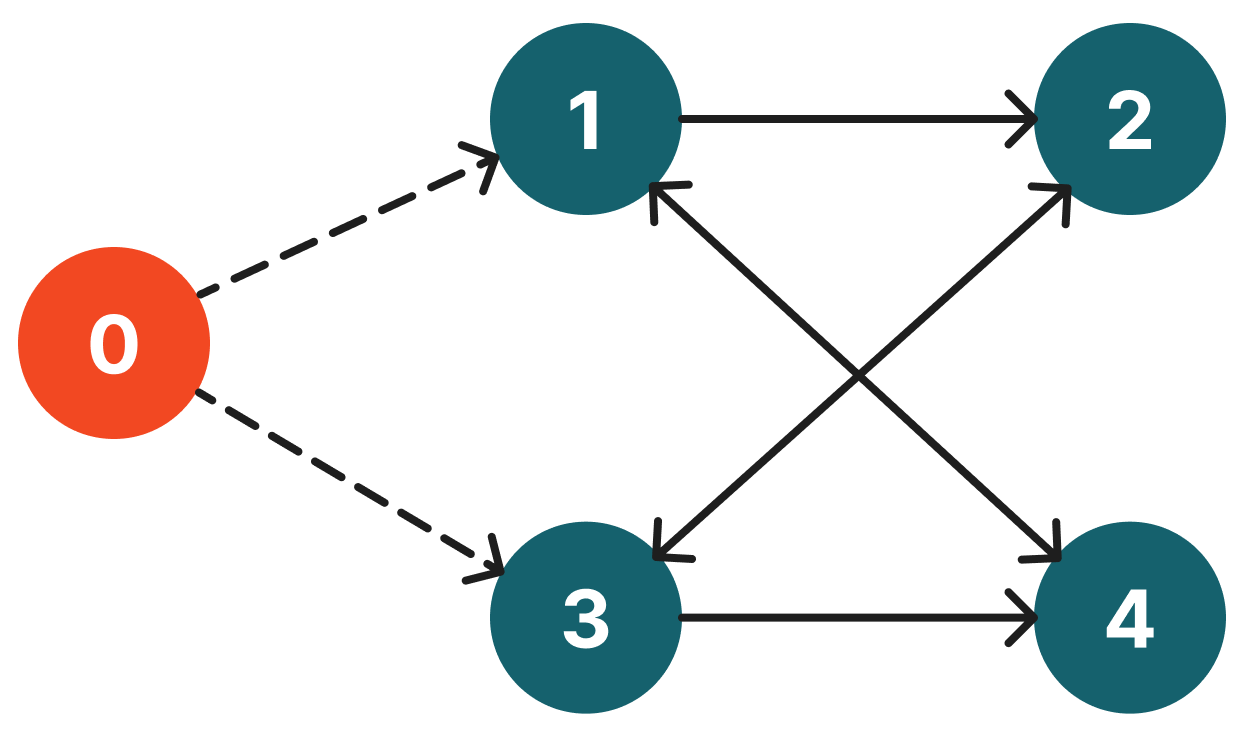
\includegraphics[width=0.6\textwidth]{communication.png}
    \caption{Communication topology among agents (DC Motors).}
    \label{fig:communication1} % Label for referencing the figure
\end{figure}

Four follower DC motors and the models for each DC motor governed by:

DC Motor 1 (Agent 1): \(y_1(k+1)=\frac{m}{rT \times 0.1} \times u_1(k)\)

DC Motor 2 (Agent 2): \(y_2(k+1)=\frac{m}{rT \times 0.1} \times u_2(k)\)

DC Motor 3 (Agent 3): \(y_3(k+1)=\frac{m}{rT \times 0.3} \times u_3(k)\)

DC Motor 4 (Agent 4): \(y_4(k+1)=\frac{m}{rT \times 0.3 } \times u_4(k)\)

In this context, \( m \) represents the total pulse count from the encoder, which measures the rotation of the motor shaft. The variable \( rT \) stands for the number of encoder counts per revolution, indicating how many counts correspond to one full rotation of the motor shaft. The variable \( T \) denotes time, which can vary and directly influences the motor's speed depending on the duration of each control input. These models are derived from the expression (\ref{model 40}).

It is evident that the agents considered are heterogeneous, as their dynamics differ from one another. In this scenario, the dynamics are assumed to be unknown and are only provided here to generate the I/O data for the multi-agent system. No model information is utilized in the distributed MFSMAC algorithm.

As illustrated in Fig. 1, the virtual leader is designated as vertex 0. It can be observed that only agents 1 and 3 can receive information from the leader, forming a strongly connected communication graph. Assume that the information exchange among agents is directed and fixed. The Laplacian matrix of the graph is given as follows:

\[
    L = \begin{bmatrix}
    1 & 0 & 0 & -1 \\
    -1 & 2 & -1 & 0 \\
    0 & -1 & 1 & 0 \\
    -1 & 0 & -1 & 2
    \end{bmatrix}
\]

with \( D = \text{diag}(1, 0, 1, 0) \). The reciprocal of the greatest diagonal entry of \( L + D \) is 0.5. By selecting the controller parameters as \( \rho = 1 \), the convergence condition in Theorem 2 and Theorem 3 is satisfied for all \( i = 1, 2, 3, 4 \). We then consider the following two distinct desired trajectories.


\subsection{Time Invariable Desired Trajectory}

where \( L + 1 \) accounts for the range from 0 to 100. The expression for \( y_d(k) \) is:

\[
y_d(k) = 0.5 \cdot \sin\left(\frac{k \pi}{30}\right) + 0.3 \cdot \cos\left(\frac{k \pi}{10}\right)
\]

for \( k \) in the range \( 0 \leq k \leq 100 \).

The initial parameters are chosen as \(u_i(1)=0.1\), \(y_i(1)=0.1\), \(\phi_i(0)=1 \) for all agents in this simulation ,\(\gamma_{1,2}=0.15\) and \(\gamma_{3,4}=0.45\),\(T=0.1\),\(m=350\), \(\eta=1\),\(\mu=1\). The MFA Controller parameters are given as \(\rho=1\),\(\lambda=50\) and the SM Controller parameters are 
\(\alpha=1\) with \(\epsilon=10^-5\).

\begin{figure}[h!]
    \centering
    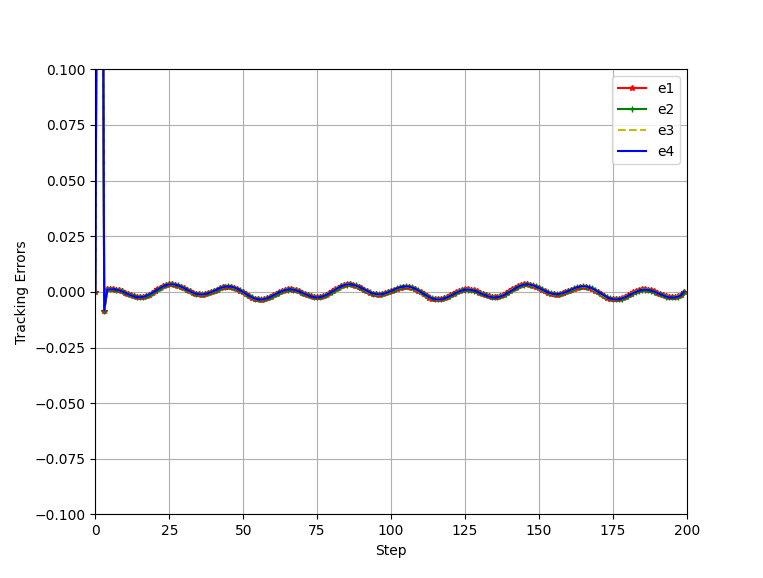
\includegraphics[width=0.6\textwidth]{Figure_2.png}
    \caption{Tracking Errors for time varying desired trajectory.}
    \label{fig:figure_2} % Label for referencing the figure

    As shown in Figure 2, the tracking errors between the actual and desired trajectories for agents a1, a2, a3, and a4 are relatively small and converge to zero over time, indicating satisfactory performance. However, the individual agents exhibit varying levels of tracking error, suggesting that their unique dynamics or initial conditions may influence their performance.
\end{figure}



\begin{figure}[h!]
    \centering
    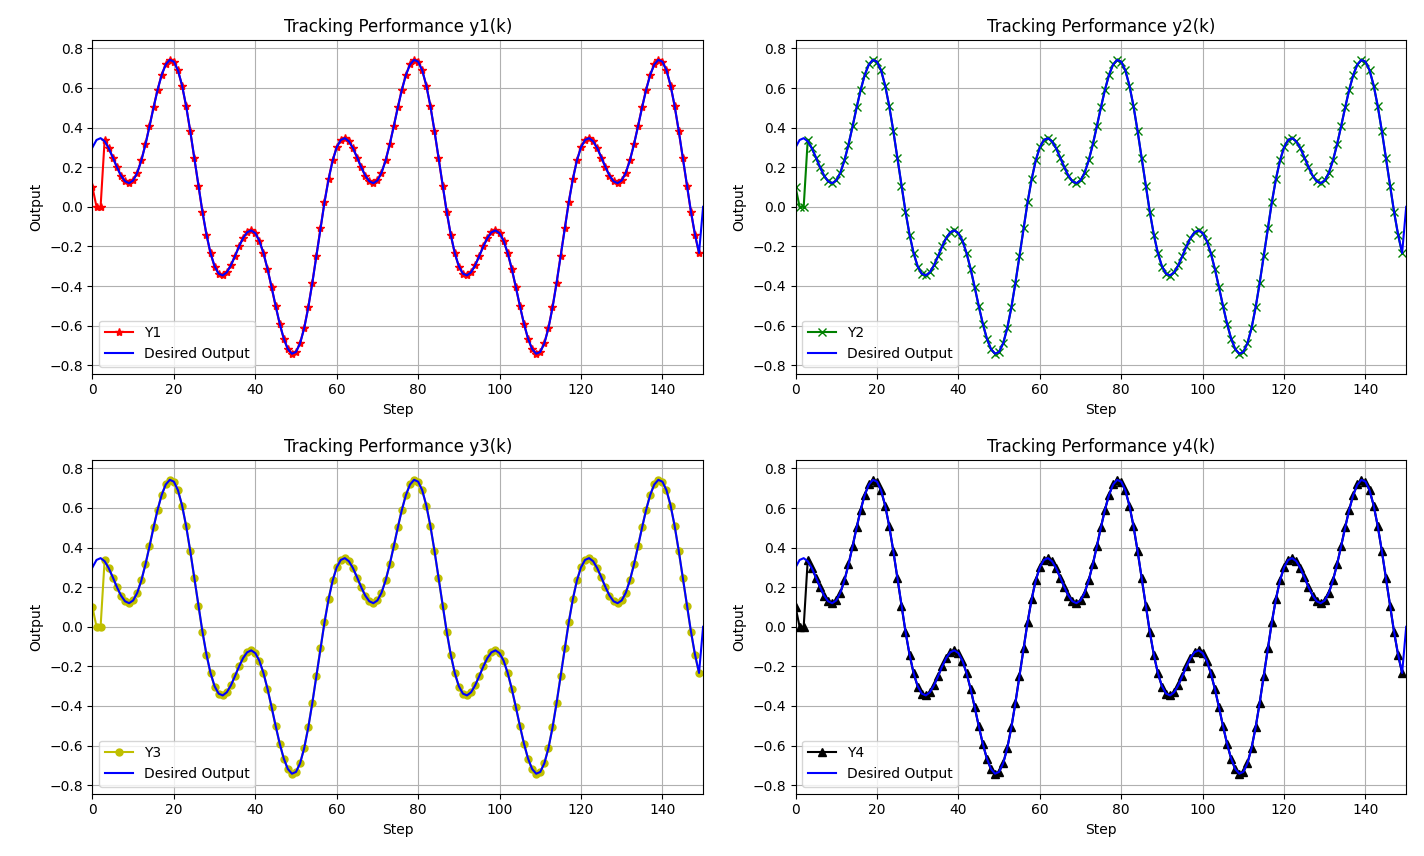
\includegraphics[width=0.7 \textwidth]{Figure_3.png}
    \caption{Tracking performance of all ageents for time varying desired trajectory.}
    \label{fig:figure_3} % Label for referencing the figure

    Figure 3 presents a detailed analysis of the tracking performance for all agents.  As illustrated, all agents successfully track the time-varying desired trajectory, confirming the effectiveness of the proposed control system. While minor variations in individual trajectories are evident, they generally adhere to the desired path. Factors such as agent dynamics, communication delays, and environmental disturbances could potentially influence the tracking performance.
\end{figure}



\begin{figure}[h!]
    \centering
    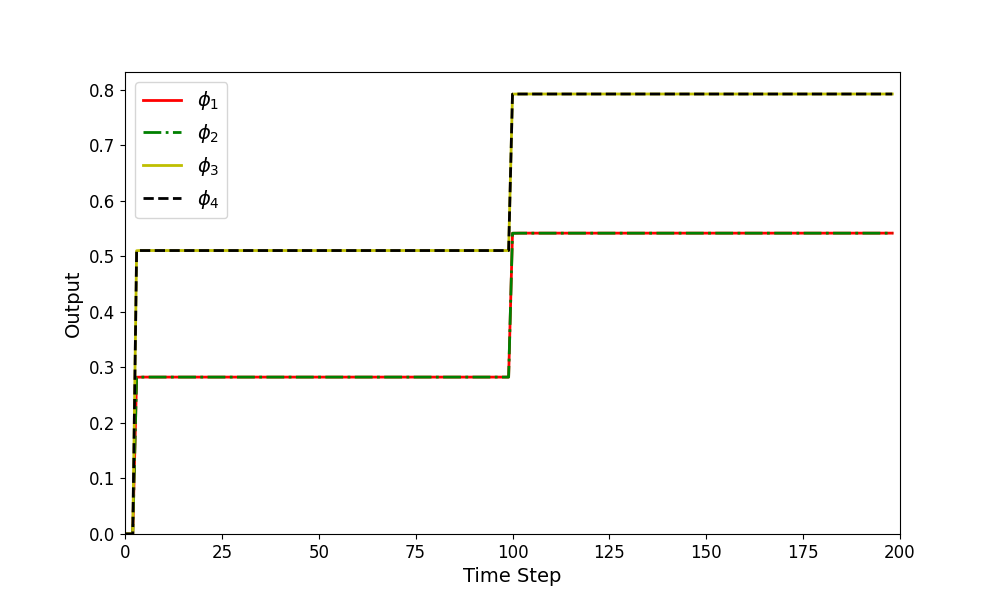
\includegraphics[width=0.6 \textwidth]{Figure_5.png}
    \caption{Tracking Errors  for time Invariable desired trajectory.}
    \label{fig:figure_4} % Label for referencing the figure
\end{figure}

\begin{figure}[h!]
    \centering
    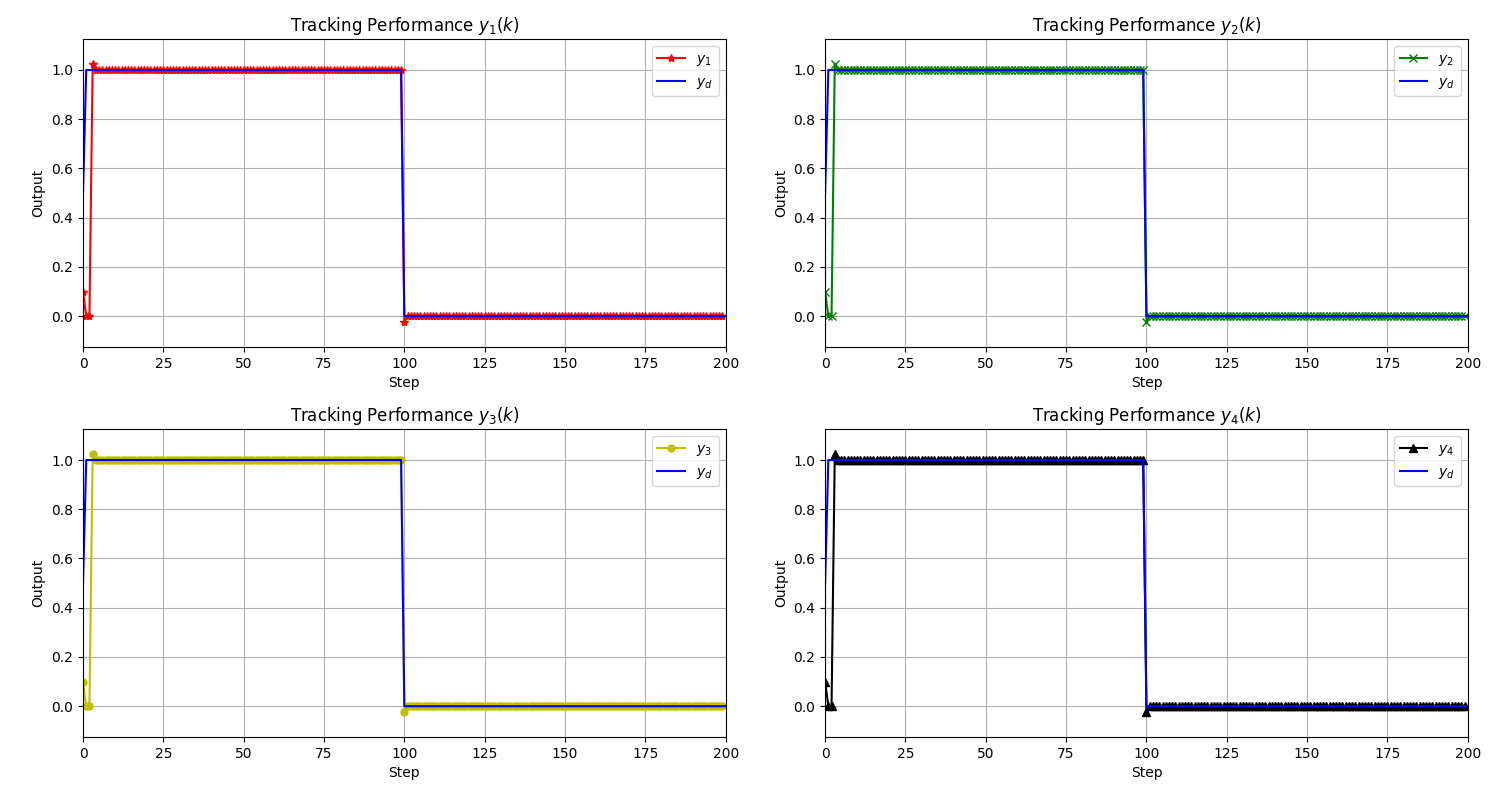
\includegraphics[width=0.7 \textwidth]{Figure_4.png}
    \caption{Tracking performance of all agents for time Invariable desired trajectory.}
    \label{fig:figure_5} % Label for referencing the figure
\end{figure}

\section{Conclusion}

This paper introduces a Model-Free Adaptiive Sliding Mode Control(MFASMC) system. The proposed approach is the speed regulation of multiple DC motors. Model-Free Adaptive Control(MFAC), combined with Sliding Mode Control(SMC), ensures a robust performance despite varying motor characteristics and uncertainties. The system utilizes a fixed topology with Laplacian matrices to effectively handle the interconnections between multiple DC motors and maintain precise speed control. This is demonstrated through the simulation results presented in figure 1 to figure 5.

 
\end{document}